\documentclass[a4paper,12pt,hidelinks]{report}

%%Pacchetti utili anche se non necessari

\usepackage{amsfonts}
\usepackage{amsmath}
\usepackage{latexsym}
\usepackage{tabularx}
\usepackage[italian]{babel}
\usepackage[bookmarks=true]{hyperref}
\usepackage{url}
% \usepackage{subfigure}
\usepackage{epstopdf}
\usepackage[utf8]{inputenc}
% \usepackage[utf8x]{inputenc}
\usepackage{listings}
\usepackage{graphicx}
%-------------------------------------------

\title{Progettazione sito web\\ ''B\&B La Vecchia Posta''}
\author{Daniele Di Pompeo \\mat. 226766}
% \annoaccademico{2013-2014}
\begin{document}
%   \begin{figure}%
% 	\includegraphics[scale=1.5,keepaspectratio=true]{img/vpLogo}%
% 	\centering
%   \end{figure}

\maketitle

%----------------------------------------------------

\chapter{Generalità}
\section{Il Committente}
Il B\&B La Vecchia Posta, innaugurato nell'Agosto del 2010 è situtato nel comune di Cagnano Amiterno, a pochi chilometri dal centro della città di L'Aquila. Situato in Via Amiternum n 6 è
stato innaugurato nell'Agosto del 2010 con la volontà e l'idea di far risvegliare dal torpidio il paese natale del committente.
Offre ai suoi clienti 6 spaziose camere tutte con bagno privato, ampio spazio verde di proprietà garantendo ai suoi clienti il massimo confort e relax. 
Si riporta una veduta aerea dell'area del B\&B per far rendere conto al lettore la posizione geografica e la conformazione dello spazio (fig.\ref{fig:bbArea}). 

\begin{figure}[h!]%
% 	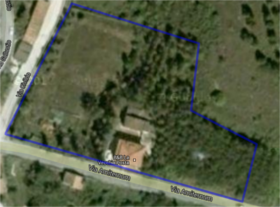
\includegraphics[width=0.6\textwidth,keepaspectratio=true]{img/bbArea1}
	\centering
	\caption{Veduta area del B\&B La Vecchia Posta}%
	\label{fig:bbArea}%
\end{figure}
L'attività del B\&B è principalmente legata al turismo primaverile/estivo in quanto il paese non offre strutture adeguate per attirare turisti invernali.
Il B\&B organizza percorsi turistici segnalando le bellezze naturali del posto, è legato al portale ``Tripadvisor'' dal quale ha ricevuto per l'anno 2012 e per l'anno 2013 il tagliando di struttura consigliata dal portale.
Il committente, che in questo particolare caso risulta essere anche lo sviluppatore dell'applicazione web, è riuscito a stringere collaborazioni con altri portali di promozione del turismo come ``Bed-and-Breakfast.it'', che risulta essere
il primo portale italiano interamente dedicato al mondo del B\&B. il B\&B risulta essere ad conduzione familiare, è gestito dal sottoscritto e con la collaborazione dei propri genitori, inoltre non ha nessun dipendente.

\section{Situazione attuale}
Il B\&B La Vecchia Posta risulta essere titolare di un dominio web dall'URL www.vecchiaposta.it, non sono stati previsti alias per il momento. il sito web è stato realizzato nel 2010 dalla Fermenti Grafici, web agency aquilana, che a titolo di amicizia ha realizzato
il comparto grafico (logo, foto, template) ed ha fornito gratuitamente e momentaneamente l'hosting. 
Ad oggi il sito web risulta essere completamente gestito dal sottoscritto ed è hostato dalla web farm ARUBA.
Sin dalla sua prima versione il sito web del B\&B è stato  realizzato utilizzando WordPress, uno dei più famosi CMS nel mondo del web e sono stati installati alcuni plug-in per fornire al sito alcune funzionalità 
di cui il committente aveva bisogno. \\
Il traffico del sito risulta essere monitorato dal servizio di google analytics, che ci ha permesso di analizzare il comportamento dell'utente su ogni singola pagina del sito web. Si riportano degli screenshot che descrivono il comportamento
dell'utenza sul sito web (fig.\ref{fig:analytics1}).

\begin{figure}[h!]
   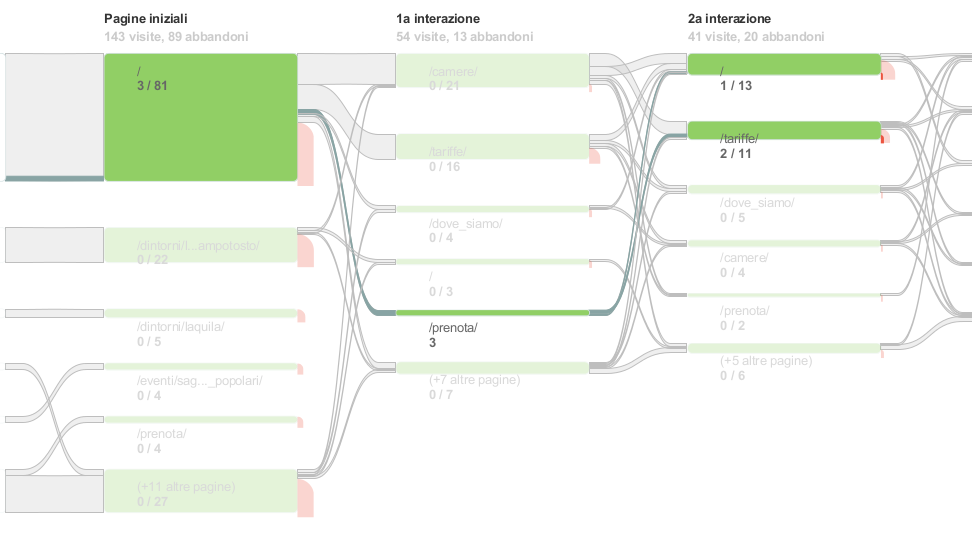
\includegraphics[width=0.8\textwidth,keepaspectratio=true]{img/googleAnalytics1}
   \centering
   \caption{Statistiche analytics}%
   \label{fig:analytics1}%
\end{figure}
Da una prima analisi dei dati raccolti dal report di google analytics risulta chiaro che la paginazione della home page risulta non essere in linea con le linee guide sulla progettazione di interfacce utente per applicazioni web.
Il traffico utente risulta non raggiungere l'obiettivo del sito web che è aumentare le prenotazioni.

\subsection{Aspetti rilevanti del sito}
Dall'analisi di alcuni test utenti effettuati su ospiti del B\&B risulta essere gradita il comporto grafico del sito, ma non è invece intuibile il meccanismo della prenotazione.
\subsection{Principali pregi}
Gli aspetti di pregio sono significativamente attribuibili all'intero comparto grafico, con scelte professionali per quanto riguarda il logo e l'accostamento di colori. Le foto utilizzate nel sito risultano essere gradevoli e
notevolmente descrittive della realtà.
\subsection{Principali difetti}
Gli aspetti negativi del sito del B\&B risultano essere legati alla progettazione della disposizione degli elementi nel display, dal fatto che il sito web non è responsive (pecca non attribuibile alla Fermenti Grafici in quanto
non richiesta inizialmente dal committente). 
Si nota dallo screenshot seguente (fig. \ref{fig:analytics2}) che gli utenti non ricevono abbastanza informazioni nella parte sopra la piega e quindi non arrivano ad effettuare prenotazioni.
\begin{figure}[h!]
  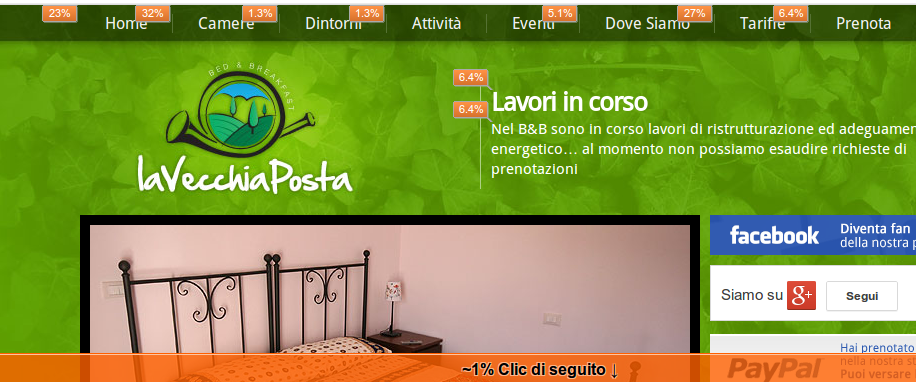
\includegraphics[width=0.9\textwidth,keepaspectratio=true]{img/googleAnalytics2}
   \centering
   \caption{Percentuali di click sulla home page}%
   \label{fig:analytics2}%
\end{figure}
Dai dati raccolti risulta che solamente un 6\% effettua click alla voce del menu ``Prenota'' e mentre meno del 1\% arriva a visionare il sito oltre la piega, effettuando quindi uno o più scroll verticali.


\section{Obiettivi generali del nuovo sito}
16. Obiettivi generali del nuovo sito, loro priorità e tempistica
17. Obiettivi specifici del nuovo sito, loro priorità e tempistica
18. Come si potrà verificare a fine progetto il raggiungimento degli obiettivi?
\section{Utenti}
\section{Scenari d'uso}
\section{Posizionamento competitivo}

%----------------------------------------------------

\chapter{Requisiti del sito}

\section{Requisiti di architettura}

\section{Requisiti di comunicazione}

\section{Requisiti funzionali}
	\subsection{Casi d'uso}
	\subsection{Base di dati}
	\subsection{Sicurezza e privacy}

\section{Requisiti di contenuto}

\section{Requisiti di gestione}
	\subsection{Infrastruttura per l'esercizio del sito}
	\subsection{Gestione dei sistemi}
	\subsection{Gestione del sito}
	\subsection{Gestione dei contenuti}
	\subsection{Getione degli utenti}

\section{Requisiti di accessibilità}
	\subsection{Prestazioni}
	\subsection{Reperibilità}
	\subsection{Compatibilità con i browser}
	\subsection{Accessibilità da parte di utenti disabili}

\section{Requisiti di usabilità}

\section{Glossario}

%----------------------------------------------------

\chapter{Requisiti di gestione progetto}

\section{Tempi e risorse}
\section{Gruppo di progetto}
\section{Responsabilità del committente}
\section{Documentazione prevista}
\section{Verifiche e convalide}
\section{Consegna finale e pubblicazione del sito}
\section{Ambiente di sviluppo}
\section{Altri requisiti}
\section{Analisi dei rischi}


\end{document}